\documentclass[conference]{IEEEtran}

\makeatletter
\usepackage{float}
\def\ps@IEEEtitlepagestyle{%
  \def\@oddfoot{\mycopyrightnotice}%
  \def\@evenfoot{}%
}
\def\mycopyrightnotice{%
  {\footnotesize 978-1-6654-6159-7/22/\$31.00~\copyright2022 IEEE\hfill}% <--- Change here
  \gdef\mycopyrightnotice{}
}
%\copyrightnotice{978-1-6654-6159-7/22/$31.00 ©2022 IEEE}

\usepackage{blindtext}
\usepackage{eso-pic}
\IEEEoverridecommandlockouts
% The preceding line is only needed to identify funding in the first footnote. If that is unneeded, please comment it out.
\usepackage{cite}
\usepackage{amsmath,amssymb,amsfonts}
\usepackage{algorithmic}
\usepackage{graphicx}
\usepackage{textcomp}
\usepackage{xcolor}
\def\BibTeX{{\rm B\kern-.05em{\sc i\kern-.025em b}\kern-.08em
    T\kern-.1667em\lower.7ex\hbox{E}\kern-.125emX}}
    
\usepackage{eso-pic}
\newcommand\AtPageUpperMyright[1]{\AtPageUpperLeft{%
 \put(\LenToUnit{0.17\paperwidth},\LenToUnit{-2cm}){%
     \parbox{0.9\textwidth}{\raggedleft\fontsize{8}{11}\selectfont #1}}%
 }}%
\newcommand{\conf}[1]{%
\AddToShipoutPictureBG*{%
\AtPageUpperMyright{#1}
}
}    
    
    
\begin{document}
\title{\vspace*{1cm} Methodology for the application of data science in breast cancer diagnosis\\
%{\footnotesize \textsuperscript{*}Note: Sub-titles are not captured in Xplore and
%should not be used}
%\thanks{Identify applicable funding agency here. If none, delete this.}
}

\author{\IEEEauthorblockN{1\textsuperscript{st} Jorge Millán}
	\IEEEauthorblockA{\textit{Facultad de ingeniería} \\
		\textit{Universidad Distrital “Francisco José de Caldas”}\\
		Bogotá, Colombia  \\
		jamillang@udistrital.edu.co}
	\and
	\IEEEauthorblockN{2\textsuperscript{nd} Edith Aparicio}
	\IEEEauthorblockA{\textit{Facultad de ingeniería} \\
		\textit{Universidad Distrital “Francisco José de Caldas”}\\
		Bogotá, Colombia \\
		eaparicio@udistrital.edu.co}
}



\maketitle
\conf{\textit{  Proc. of the Interdisciplinary Conference on Mechanics, Computers and Electrics (ICMECE 2022)  \\ 
6-7 October 2022, Barcelona, Spain}}
\begin{abstract}
In 2020 the detected cases of breast cancer in Colombia were 15,509 of which 4,411 ended in death. The anticipate prognosis of this disease has become a research need because it can facilitate preventive treatment to avoid its lethality in an advanced stage. This paper proposes the DSM-BCD methodology (Data science methodology for breast cancer diagnosis) designed to speed up the diagnosis of breast cancer through the continuous improvement of Machine Learning and Deep Learning techniques based on the insight of the oncology specialist and the feedback of knowledge according to the behavior of the data in the various techniques for the detection of breast cancer. 
\end{abstract}

%\copyrightnotice{978-1-6654-6159-7/22/$31.00 ©2022 IEEE}


\begin{IEEEkeywords}
Methodology, Data Science, Breast Cancer, Diagnostics, Machine Learning, Deep Learning
\end{IEEEkeywords}


\section{INTRODUCTION}

In 2020, the number of cases of breast cancer worldwide amounted to 2,261,419 and 684,996 of these cases ended in death. In Colombia, there were 15,509 cases and 4,411 deaths \cite{InternationalAgencyforResearchonCancer2020}, ranking first in the lethality rate among all types of cancer affecting women of all ages. This type of cancer originates when breast cells begin to grow out of control becoming malignant cells that usually form a tumor that can often be seen on an x-ray or can be palpated as a mass or lump \cite{Sauer2019}. Colombia has limitations with respect to access to early detection and diagnosis of cancer, caused in most cases by factors such as socio-economic status, health insurance coverage, origin and accessibility. On average, the waiting time for a patient is 90 days from the onset of symptoms to the diagnosis of cancer. The first action to reduce the mortality rate from breast cancer should be focused on the speed of diagnosis and timely access to care\cite{Duarte2021}. Early prognosis of this disease has become a research need because it may facilitate preventative treatment to avoid its progression lethality in an advanced stage. An alternative to reduce this mortality rate is to be able to predict and identify, based on the analysis of a set of data obtained from examinations performed by various medical methods to the individual, what is the probability of contracting breast cancer and what are the variables that most influence the suffering of this disease, and according to these results provide a preventive treatment to combat cancer before it metastasizes or reaches an advanced stage where it is more difficult to treat.

The analysis obtained through data science allows detecting cancer in a shorter time, because ML (Machine Learning) and DL (Deep Learning) algorithms clearly impact exploratory studies that aim to identify the biological principles of the disease which can benefit patients and physicians by speeding up diagnosis and providing support to make better and faster decisions at the clinical level\cite{Turin2020}. In recent years, the increase in computer power, coupled with mathematical advances, has enabled the use of multilayer (deep) complex neural networks which have improved the performance of automatic interpretation of highly standardized oncological images\cite{Mann2020}.

On the other hand, science, in the language of the scientific method, is to formulate hypotheses or conjectures based on observations of the world around us in order to validate or invalidate those hypotheses by conducting experiments. However, unlike the pure sciences, working with data does not necessarily require conducting experiments. Rather, often the data have already been collected and organized previously. So, the scientific method, applied to data, can be summarized as: \textit{“Formulate hypotheses based on the world around us and then analyze the relevant data to validate or invalidate those hypotheses”}.

Data science is currently used by different researchers to model the progression and treatment of cancerous conditions because of its ability to detect significant features in complex data sets. Data-driven medicine has the ability not only to improve the speed and accuracy of diagnosis of genetic diseases, but also to unlock the possibility of personalized medical treatments\cite{Baker2018}. To learn means: \textit{“To acquire knowledge or skills in something through experience”}. Therefore, ML could be framed as the way in which a machine gains or acquires knowledge through experience. But, how does a machine gain experience? All inputs to a machine are essentially binary strings of 0 and 1, which in the domain of computer science are simply data. Therefore, ML is really the way a computer acquires knowledge through data. \\

Data science is fundamentally a process, while ML is a tool that can be immensely useful in carrying out that process\cite{Pillai2020}. Of course, this does not give any idea of the how at all; it simply summarizes the process as something that is done with the input data to generate this knowledge as output. To make a mathematical analogy, ML is a function $f$ such that:

\begin{equation}
	knowledge = f(Data)
\end{equation}

It should also be mentioned that a methodology is a general strategy that serves as a guide for the processes and activities that are within a given domain. Methodology does not rely on specific technologies or tools, nor is it a set of techniques or recipes. Rather, methodology provides the data scientist with a framework for how to proceed with the methods, processes and arguments that will be used to obtain answers or results\cite{Rollins2015}.
Thus, the objective of this paper is to propose a methodology in data science for the diagnosis of breast cancer, this with the purpose of applying the use of this computational science as a multidisciplinary field that allows to give value to the data obtained through medical techniques for the diagnosis of breast cancer through a process that facilitates the analysis and selection of techniques in order to make a decision that validates the veracity of a hypothesis raised. The use of the proposed methodology has an impact on the ease of obtaining data and processing information for the diagnosis and prognosis of this disease.

\section{BREAST CANCER SCREENING AND DIAGNOSIS}
Breast cancer, with its uncertain cause, has captured the attention of surgeons throughout the ages. Despite centuries of theoretical mazes and scientific questions, breast cancer is still one of the most dreaded human diseases\cite{Bland2009}. According to \cite{Fatima2020}, breast cancer originates through malignant tumors, when the cell growth gets out of control causing many fatty tissues and fibrous tissues of the breast initiate abnormal growth, which results in cancer cells spreading through the tumors causing the different stages of cancer. \cite{Fatima2020} state that there are different types of breast cancer, which occur when the affected cells and tissues spread throughout the body \cite{Sun2017}. For example, the first type of cancer called \textit{Ductal Carcinoma in situ (DCIS)} is a non- invasive type of cancer\cite{Hou2020}, which occurs when abnormal cells spread outside the breast. The second type of cancer is \textit{Invasive Ductal Carcinoma (IDC)}, also known as infiltrating ductal carcinoma \cite{Chaudhury2011}. This type of cancer occurs when abnormal breast cells spread throughout the breast tissues. Usually, this type of cancer is found in men \cite{Page1982}. The third type of cancer is \textit{Mixed Tumor Cancer (MTBC)} also known as invasive breast cancer\cite{Tuck1997}  caused by abnormal duct cells and lobular cells\cite{Lee2017}. The fourth type of cancer is \textit{Lobular Breast Cancer (LBC)}\cite{Masciari2007}  which occurs within the lobule and increases the chances of other invasive cancers. The fifth type of cancer is \textit{Mucinous Breast Cancer (MBC)} or \textit{Colloid Breast Cancer}\cite{Memis2000} that occurs due to invasive ductal cells when abnormal tissue spreads around the duct \cite{Gradilone2011}. The sixth and last type of cancer is \textit{Inflammatory Breast Cancer (IBC)}, which causes swelling and redness of the breast. This type of breast cancer is fast growing, and begins to appear when lymphatic vessels become clogged in ruptured cells \cite{Robertson2010}. According to \cite{Brunicardi2010}, in the majority of detected cases the woman discovers a lump in her breast. Other signs and symptoms that occur less often include: breast growth or asymmetry, nipple alterations and retraction or telorrhea, ulceration or erythema of the breast skin, an axillary mass, and musculoskeletal discomfort. It should be noted that if any of the above symptoms are detected, this type of cancer can be detected by means of procedures based on \textit{physical examination}, \textit{imaging techniques} and \textit{biopsies}. At the physical examination level, breast cancer can be detected by the oncologist using the methods of \textit{inspection} and \textit{palpation}. With these methods, the symmetry, size and shape of the breast are recorded, as well as any evidence of edema (orange peel), nipple or skin retraction and erythema \cite{Brunicardi2010}. Currently, many \textit{imaging techniques} are widely used to provide an accurate diagnosis of breast lesions \cite{Tamam2021}, among these techniques the most relevant are the following: \textit{Mammography} which makes use of a mammographic unit consisting of an X-ray tube encapsulating a cathode and an anode. The breast is placed on the detector and is compressed by a device of parallel plates, which keeps the breast immobile and prevents blurring by movement, this in order to reduce the thickness of the tissue that must pass through the X-rays \cite{Ebrahimi2019}; \textit{Ductography} that identifies lesions in patients with nipple discharge. This method is effective in localizing and identifying intraductal lesions by means of a mammographic examination performed after retrograde filling of the lactiferous ducts with contrast material \cite{Hirose2007}; \textit{Ultrasound}, which allows high-resolution images to be obtained by means of a small high- frequency transducer (tube) that sends inaudible sound waves into the breast and receives the echo of waves from internal organs, fluids and tissues \cite{Hasan2019}; and \textit{Magnetic Resonance Imaging (MRI)}, which is used when breast lesions cannot be easily assessed by other techniques. To achieve this, it uses radiofrequency (RF) receiver coils to detect a signal emitted by tissues upon excitation of an electromagnetic field that forces protons to align to the anatomy of the area of interest in size and shape \cite{Tse2014}. It should also be mentioned that there are currently there are two ways to obtain a diagnosis by \textit{biopsy} for a patient with a breast abnormality. On the one hand we have the biopsy for breasts with p\textit{alpable lesions} also called \textit{percutaneous} or \textit{minimally invasive}. These biopsies include Fine Needle Aspiration (FNA) and Core Needle Aspiration (CNB). Open surgical biopsies are sometimes referred to as excisional biopsies or incisional biopsies. \textit{Excisional} biopsy indicates complete removal of the lesion, whereas \textit{incisional} biopsy indicates removal of part of the lesion \cite{Greenfield2012}. For nonpalpable lesions, imaging modalities such as ultrasound (US), mammography, and magnetic resonance imaging (MRI) are useful adjuncts to identify and localize the lesion of interest. The decision of when to perform a breast biopsy depends on the patient's history, physical examination findings, and radiologic imaging. The primary goal of biopsy is to obtain a tissue diagnosis that can help dictate treatment and preoperative planning, if indicated. Therefore, it is imperative to choose a biopsy technique that optimizes the chances of obtaining an accurate diagnosis while minimizing costs, limiting patient discomfort and reducing the need for repeat procedures\cite{Samilia2018}.

\section{Data science methodology for breast cancer diagnosis (DSM-BCD)}
A systematic review was conducted in the scientific literature of various methodologies, which although they cover the necessary process for data analysis, they do not generate sufficient value for the solution of a given problem. For this reason, authors such as \cite{Martinez2021} consider that although the data science research community is growing day by day, it is exploring new domains, creating new specialized roles and is making a great research effort to develop advanced analysis, improving models and generating new algorithms supported from the fields of mathematics, statistics and computer science, these skills are not sufficient for application in real projects, since most data-driven projects present organizational and socio-technical problems, such as: a lack of vision and clarity of purpose, a biased emphasis on technical issues, and role ambiguity. And while these problems exist in real-world data science projects, the community has not been too concerned about them and not enough has been written about solutions to address these problems. Given the problems presented by data-driven projects, and the study of various methodologies proposed by several authors, the DSM-BCD (Data science methodology for breast cancer diagnosis) methodology is proposed. This methodology is based on the agile manifesto applied to a context of data-driven results. 

\begin{figure*}
	\centering
	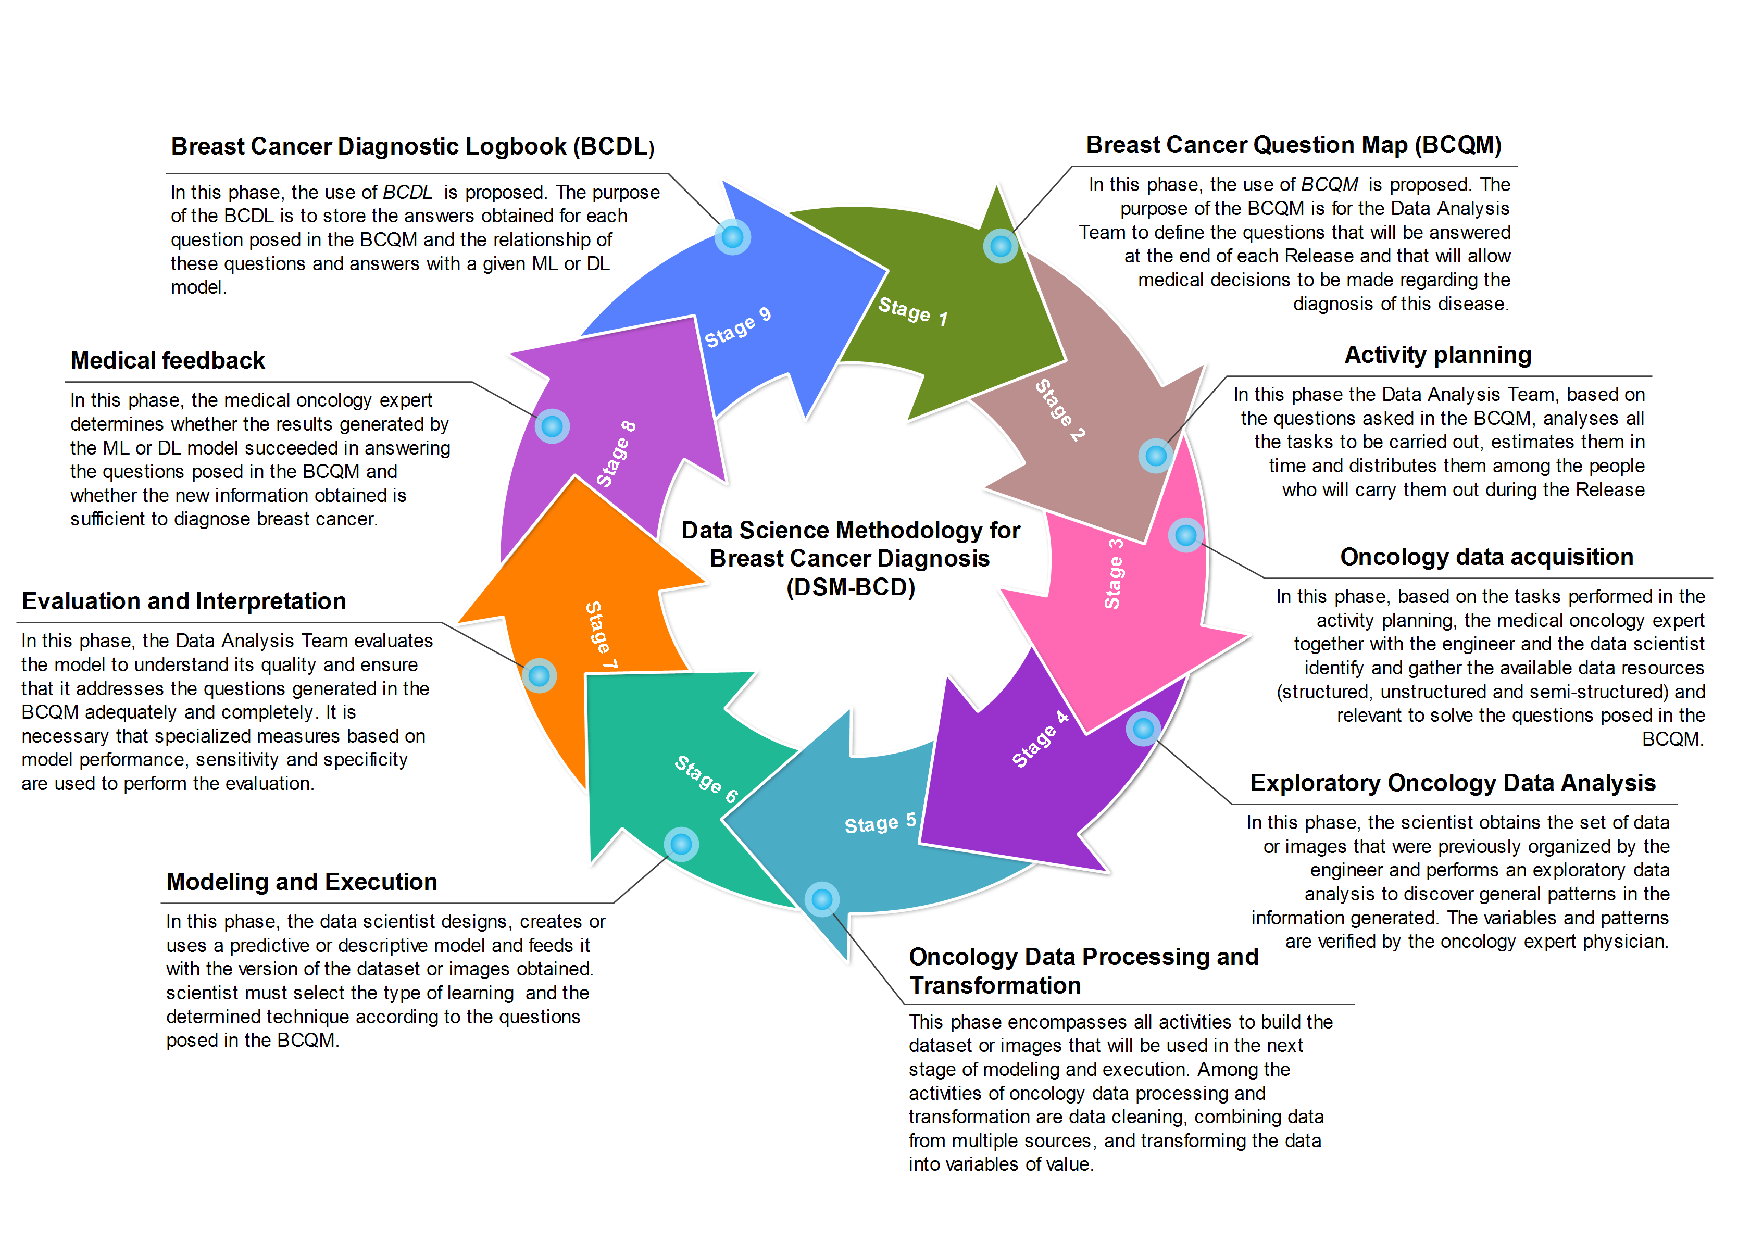
\includegraphics[width=0.9
	\linewidth]{IMAGES/DSM-BCD.pdf}
	\caption{Data science methodology for breast cancer diagnosis (DSM-BCD)}
	\label{DSM-BCD}
\end{figure*}

Given the above, DSM- BCD does not focus on evaluating the accuracy of ML and DL techniques but its main objective is to generate value to the data in the shortest possible time for physicians to diagnose breast cancer in an agile way. To achieve this, DSM-BCD integrates the medical insight and the results obtained by ML and DL techniques in continuous feedback generated in each Release to produce more efficient decision making. In DSM-BCD, a Data Analysis Team is proposed. This team should be headed by the medical oncology expert, at least one data engineer and one data scientist. It is recommended that the team be made up of a maximum of 5 people to facilitate teamwork and internal communication. Figure \ref{DSM-BCD} shows the phases of DSM-BCD. 

\subsection*{Stage 1: Breast Cancer Question Map (BCQM)} 
In this phase, the use of a Breast Cancer Question Map (BCQM) is proposed. The purpose of the \textit{BCQM} is for the \textit{Data Analysis Team} to define the questions that will be answered at the end of each \textit{Release} and that will allow medical decisions to be made regarding the diagnosis of this disease. The BCQM allows you to ask questions related to the types of breast cancer and techniques for breast cancer diagnosis. So that at the end of the time of each Release, which can vary between 1 and 4 weeks, the question will be answered according to the data analysis generated, and the doctor will be able to make a valuable decision. It should be noted that it is possible to have one or more questions related to a technique and a type of breast cancer for each Release, which is why it is possible to find correlations between the characteristic variables of each type of cancer, thus finding hidden patterns in the different data sets. Additionally, the BCQM allows to identify which technique for the diagnosis of breast cancer is related to the question to be solved, which in advance makes it possible to know the type of information (images or data) and the ML or DL algorithm required to solve the problem. Likewise, the BCQM allows to define from the initial phase the type of predictive or descriptive model according to the analytical approach generated by the question posed. Summarizing, the use of BCQM facilitates the understanding of the medical problem and allows to previously identify the technique, the type of information and approach to be used for data analysis. Figure \ref{BCQM} shows the structure of the BCQM.

\begin{figure}[H]
	\centering
	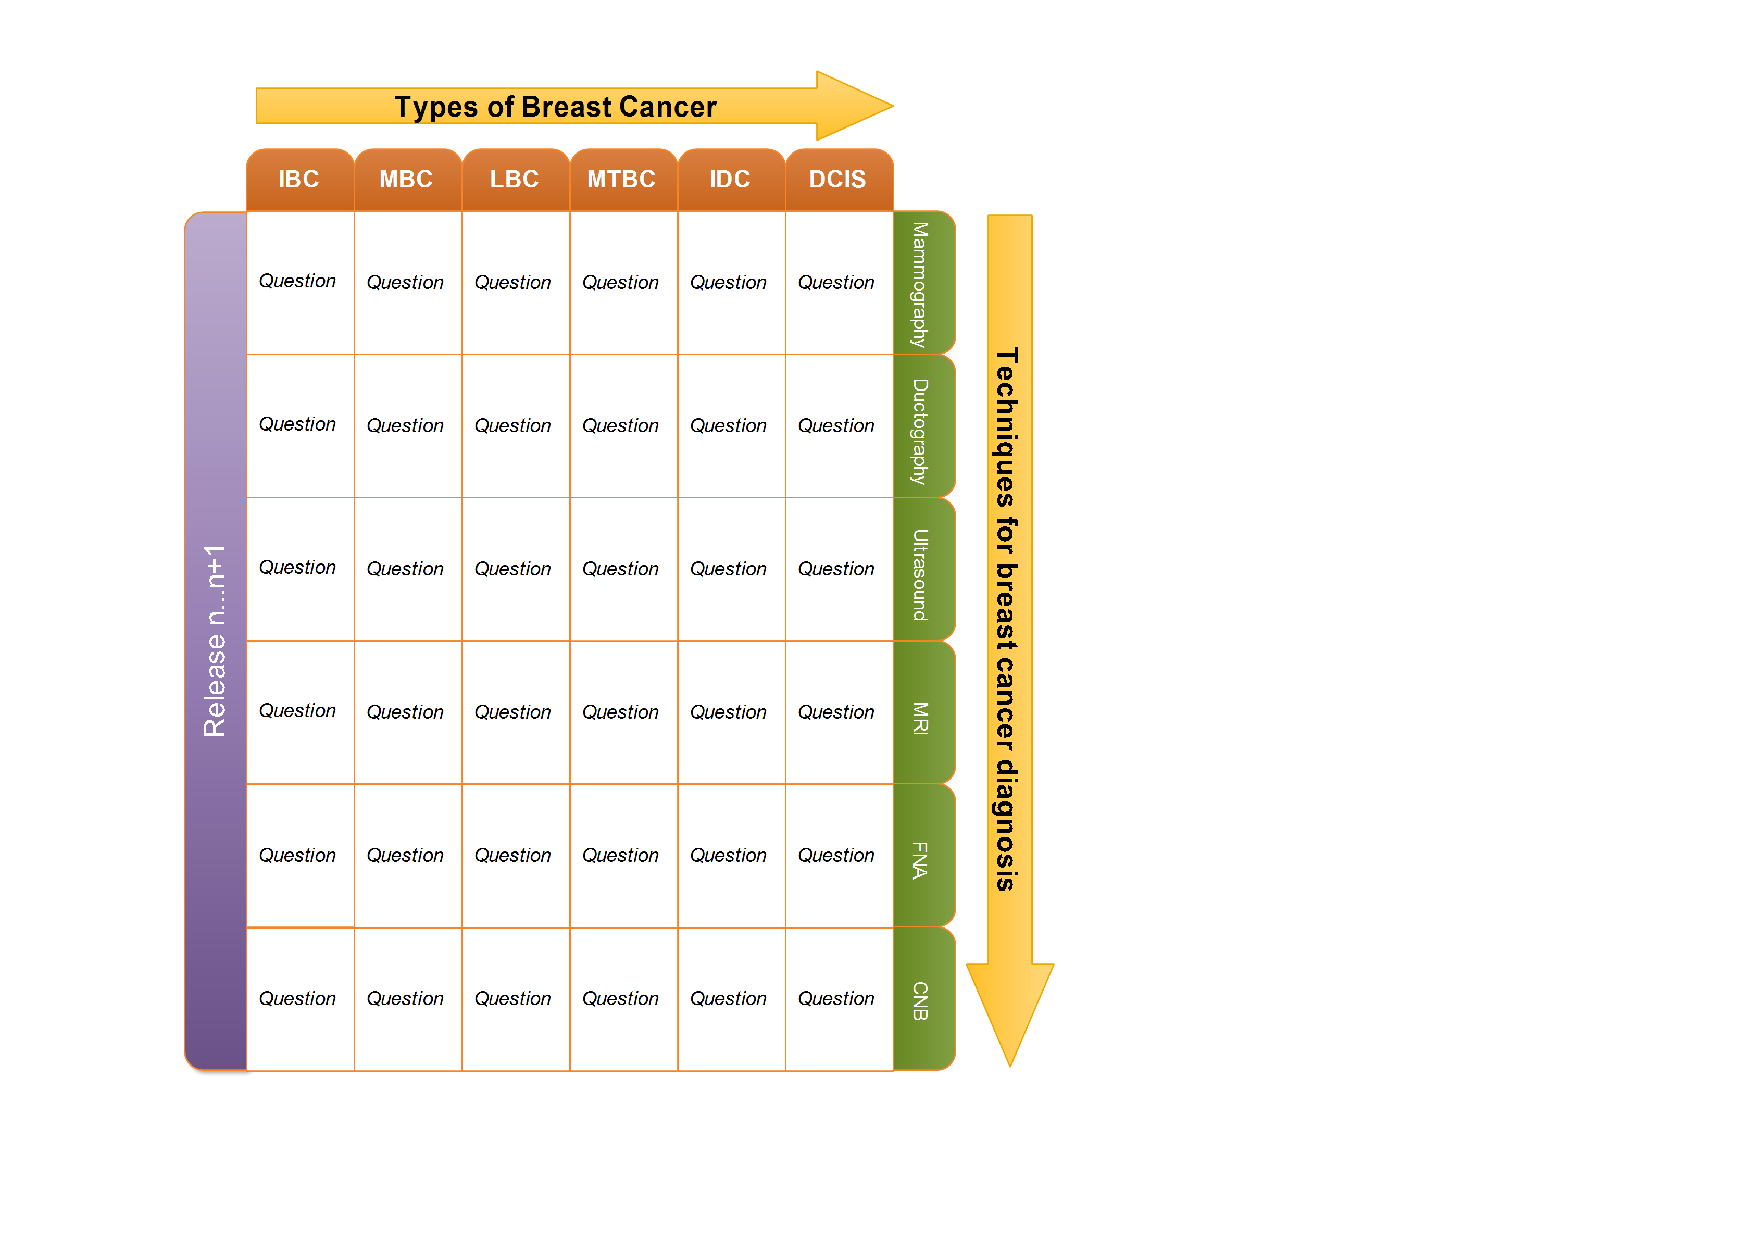
\includegraphics[width=1
	\linewidth]{IMAGES/BCQM.pdf}
	\caption{Map of questions based on inflammatory (IBC), mucinous (MBC), lobular (LBC), mixed tumour (MTBC), invasive ductal carcinoma (IDC) and ductal carcinoma in situ (DCIS) breast cancers.Map of questions based on inflammatory (IBC), mucinous (MBC), lobular (LBC), mixed tumour (MTBC), invasive ductal carcinoma (IDC) and ductal carcinoma in situ (DCIS) breast cancers.}
	\label{BCQM}
\end{figure}

\subsection*{Stage 2: Activity planning }
In this phase the Data Analysis Team, based on the questions asked in the BCQM, analyses all the tasks to be carried out, estimates them in time and distributes them among the people who will carry them out during the Release. Since the BCQM allows us to know in advance the type of breast cancer and the technique for the diagnosis of this disease, the data scientist with the help of the physician can define the data source, which will allow to know the type, quantity and weight of the information. Given the above, it is recommended that the team has at least one data engineer, since he is the one in charge of taking the data and converting it to the data source into meaningful information for the scientist to perform the respective analysis. 

\subsection*{Stage 3: Oncology data acquisition }
In this phase, based on the tasks performed in the activity planning, the medical oncology expert together with the engineer and the data scientist identify and gather the available data resources (structured, unstructured and semi-structured) and relevant to solve the questions posed in the BCQM. It should be noted that in the DSM-BCD methodology it is feasible to have several datasets or images that are related to one type of breast cancer and one diagnostic technique, therefore the Data Analysis Team can have several data scientists answering different questions in the same Release. As a consequence, in the end, multiple answers and a possible correlation between the various oncological variables can be obtained as a result. Also, in this phase the Data Analysis Team must define the necessary data infrastructure according to the amount of information to be processed, which will allow projecting the scalability, scope and distribution of such information. \\ \\

\subsection*{Stage 4: Exploratory Oncology Data Analysis }
In this phase, the scientist obtains the set of data or images that were previously organized by the engineer and performs an exploratory data analysis to discover general patterns in the information generated. It should be noted that in this phase the accompaniment of the medical expert in oncology is of vital importance, since the data or images to be explored by the scientist may contain variables that may or may not have a significant value for the expert, thus helping to determine whether or not the analysis proposed to answer the question is on the right track, so it is possible that several variables are added or eliminated to achieve the expected result. Additionally, it is necessary that the various analyses generated are supported with graphs that are understandable by the entire Data Analysis Team, this for the purpose of providing ideas, and from this phase to find possible correlations between oncological variables.

\subsection*{Stage 5: Oncology Data Processing and Transformation }
This phase encompasses all activities to build the dataset or images that will be used in the next stage of modeling and execution. Among the activities of oncology data processing and transformation are data cleaning, combining data from multiple sources, and transforming the data into variables of value. In this phase, teamwork and continuous communication between the data engineer and data scientist is important to address invalid or missing values, remove duplicates, format, and combine files, tables, and platforms. Additionally, the physician Oncology expert must provide a clearance to proceed with the next phase. This is because the domain expert has a deeper knowledge of the variables or images that are being observed, and if there is unnecessary information for the diagnosis of breast cancer, it is possible to debug that information so that it does not affect the training and subsequent execution of the ML and DL model.

\subsection*{Stage 6: Modeling and Execution}
In this phase, the data scientist designs, creates or uses a predictive or descriptive model and feeds it with the version of the dataset or images obtained in the processing and transformation phase. In this phase, the scientist must select the type of learning (supervised, unsupervised and reinforcement learning) and the determined technique (regression, classification, clustering, CNN, RNN, etc.) according to the questions posed in the BCQM. It is worth mentioning that in this phase the Data Analysis Team must define together with the oncology expert physician the error tolerance allowed in the model, given that the sensitivity of the analysis may vary depending on the type of breast cancer and the diagnostic technique. It is likely that the data scientist will try multiple algorithms with their respective parameters to find the best model for the oncological variables available. It should be noted that it is vitally important that the proposed models do not have problems of over-fitting or under-fitting as this can lead to misleading or insignificant results. Additionally, the data scientist in question together with the Data Analysis Team must define the infrastructure at the server level necessary for training and testing the model according to the amount of information to be processed, with the purpose of generating accurate results in the shortest possible time in order to fulfill the tasks defined in the planning phase of activities and give value to the oncological data once the Release is completed.

\subsection*{Stage 7: Evaluation and Interpretation}
In this phase, the Data Analysis Team evaluates the model to understand its quality and ensure that it addresses the questions generated in the BCQM adequately and completely. It is necessary that specialized measures based on model performance, sensitivity and specificity are used to perform the evaluation. Additionally, the results obtained must be understandable to the oncology physician, ensuring that the results are correctly interpreted and related to breast cancer staging and biomarkers. It is important that the physician and the data scientist adjust the model as needed. Since we are working with sensitive medical data, it is necessary that the final model is applied to a validation set for a final evaluation. In addition, the Data Analysis Team can assign to the model tests of statistical significance as an additional test to check the answer obtained to the generated question. This additional test is essential to justify the implementation of the model. Finally, since the BCQM can ask multiple questions related to different types of breast cancer and diagnostic techniques during the Release, it is necessary for the scientists with the help of the data engineer to join, if possible, the results obtained in a matrix or heat map to identify the correlation coefficient between two or more oncologic variables. This resulting matrix should be analyzed by the medical oncology expert to determine if there is a significant relationship between the different types of breast cancer.
 
\subsection*{Stage 8: Medical feedback}
In this phase, the medical oncology expert determines whether the results generated by the ML or DL model succeeded in answering the questions posed in the BCQM and whether the new information obtained is sufficient to diagnose breast cancer or whether these results generated relevant information to determine the cause or origin of this disease, in short, whether the analyzed data produced added value to the medical domain. In the case that the results obtained did not provide value to the data, the Data Analysis Team will have to decide if it is necessary to re-state the questions or if new data should be acquired to adjust the generated model. In addition, the expert in the company of the data scientist and data engineer, based on their medical acumen, should help decide which strategy is most appropriate to generate meaningful results. Similarly, if the result was satisfactory, the physician should issue an opinion on the level of impact that the information generated by the models had in diagnosing the condition of breast cancer in a given patient and once the information is verified, together with the Data Analysis Team, feed a dataset with the information obtained from the diagnoses generated for each individual. The above with the purpose of improving the performance of existing models and increase their accuracy. Finally, in each Release it must be guaranteed that the diagnosis time is shorter and shorter or that new information is generated that the doctor can use in his daily functions and that helps to determine the origin, relationship or possible treatment of this disease.

\subsection*{Stage 9: Breast Cancer Diagnostic Logbook (BCDL)}
In this phase, the use of a Breast Cancer Diagnostic Logbook (BCDL) is proposed. The purpose of the \textit{BCDL} is to store the answers obtained for each question posed in the BCQM and the relationship of these questions and answers with a given ML or DL model. This log should only be fed when the information obtained generated added value to the medical domain. Its main purpose is to avoid redundancy of information and duplication of questions posed in the BCQM, ensuring that new knowledge related to breast cancer is generated in each Release. It is recommended that the logbook be designed by means of an entity- relationship model (MER) that is made up of entities such as: model, type of breast cancer, diagnostic technique, data set, question and answer. Given the above, it is suggested that the different data sets or images used in the analysis be stored in a cloud-based information hosting service (Amazon Cloud, Google Drive, One Drive, etc.) and that this information be identified with a unique code that facilitates its search when required. Similarly, the different algorithms generated must be stored in a version control system (GitLab, GitHub, Bitbucket, etc.) with their respective operation readme and a unique identification code so that it can be easily consulted by database. Therefore, the use of the BCDL allows to have a detailed traceability of the advances obtained in each Release with respect to the diagnosis of breast cancer, this with the purpose that the Data Analysis Team has a solid starting point to innovate in new ML and DL models through the comparison and continuous improvement of existing models that managed to add value to the different types of oncological data.
\section{Conclusion}
Because that data science is a multidisciplinary field which incorporates computational tools that allow to give value to the data and learn from them in order to make a decision that validates the veracity of a hypothesis raised, it is the best option to generate a meaningful diagnosis in the detection of this disease. Given the above, although most researchers have put their efforts into breast cancer diagnostics and prognostics, each technique has a different accuracy rate that varies according to the different situations, tools and datasets being used. As data analytics capabilities become more accessible and prevalent, data scientists can find great support in the DSM-BCD methodology because it provides a guiding strategy, independent of the technologies, data volumes or approaches involved, and enables improved performance of ML and DL models to ensure agile and effective diagnosis of breast cancer.

\bibliographystyle{IEEEtran}
\bibliography{REFERENCES/articulos}
\end{document}
